%----------------------------------------------------------------------------------------
%	PACKAGES AND OTHER DOCUMENT CONFIGURATIONS
%----------------------------------------------------------------------------------------

\documentclass[11pt]{scrartcl} % Font size

%%%%%%%%%%%%%%%%%%%%%%%%%%%%%%%%%%%%%%%%%
% Wenneker Assignment
% Structure Specification File
% Version 2.0 (12/1/2019)
%
% This template originates from:
% http://www.LaTeXTemplates.com
%
% Authors:
% Vel (vel@LaTeXTemplates.com)
% Frits Wenneker
%
% License:
% CC BY-NC-SA 3.0 (http://creativecommons.org/licenses/by-nc-sa/3.0/)
% 
%%%%%%%%%%%%%%%%%%%%%%%%%%%%%%%%%%%%%%%%%

%----------------------------------------------------------------------------------------
%	PACKAGES AND OTHER DOCUMENT CONFIGURATIONS
%----------------------------------------------------------------------------------------

\usepackage{amsmath, amsfonts, amsthm} % Math packages

\usepackage{listings} % Code listings, with syntax highlighting

\usepackage{graphicx} % Required for inserting images

\usepackage{booktabs} % Required for better horizontal rules in tables

\usepackage{dirtytalk} % Required for quoting.

\usepackage{float} % Added for hard placement of images.

\usepackage[dvipsnames]{xcolor} % Added for extra colors.

\usepackage{tikz} % For colored boxes and more.

\numberwithin{equation}{section} % Number equations within sections (i.e. 1.1, 1.2, 2.1, 2.2 instead of 1, 2, 3, 4)
\numberwithin{figure}{section} % Number figures within sections (i.e. 1.1, 1.2, 2.1, 2.2 instead of 1, 2, 3, 4)
\numberwithin{table}{section} % Number tables within sections (i.e. 1.1, 1.2, 2.1, 2.2 instead of 1, 2, 3, 4)

\usepackage{enumitem} % Required for list customisation
\setlist{noitemsep} % No spacing between list items

\usepackage[main=greek, english]{babel}

%----------------------------------------------------------------------------------------
%	DOCUMENT MARGINS
%----------------------------------------------------------------------------------------

\usepackage{geometry} % Required for adjusting page dimensions and margins

\geometry{
	paper=a4paper, % Paper size, change to letterpaper for US letter size
	top=2.5cm, % Top margin
	bottom=3cm, % Bottom margin
	left=3cm, % Left margin
	right=3cm, % Right margin
	headheight=0.75cm, % Header height
	footskip=1.5cm, % Space from the bottom margin to the baseline of the footer
	headsep=0.75cm, % Space from the top margin to the baseline of the header
	%showframe, % Uncomment to show how the type block is set on the page
}

%----------------------------------------------------------------------------------------
%	FONTS
%----------------------------------------------------------------------------------------

\usepackage[utf8]{inputenc} % Required for inputting international characters
\usepackage[T1]{fontenc} % Output font encoding for international characters

\usepackage{XCharter} % Use the XCharter fonts


%----------------------------------------------------------------------------------------
%	SECTION TITLES
%----------------------------------------------------------------------------------------

\usepackage{sectsty} % Allows customising section commands

\sectionfont{\vspace{6pt}\centering\normalfont\scshape} % \section{} styling
\subsectionfont{\normalfont\bfseries} % \subsection{} styling
\subsubsectionfont{\normalfont\itshape} % \subsubsection{} styling
\paragraphfont{\normalfont\scshape} % \paragraph{} styling

%----------------------------------------------------------------------------------------
%	HEADERS AND FOOTERS
%----------------------------------------------------------------------------------------

\usepackage{scrlayer-scrpage} % Required for customising headers and footers

\ohead*{} % Right header
\ihead*{} % Left header
\chead*{} % Centre header

\ofoot*{} % Right footer
\ifoot*{} % Left footer
\cfoot*{\pagemark} % Centre footer

\newcommand{\img}[1] % maybe add a caption to this
{
    \begin{center}
        \fcolorbox{black}{white}{\includegraphics[width=\textwidth]{#1}}
    \end{center}

}

% Helper Macros

\newcommand{\en}[1]{\foreignlanguage{english}{#1}}
\newcommand{\src}[1]{{\texttt{#1}}}


% Extra Formatting

\setlength{\parindent}{0em}
\setlength{\parskip}{0em}


% Code Listing Style

\lstdefinestyle{code}{
  belowcaptionskip=1\baselineskip,
  breaklines=true,
  frame=LRTB,
  xleftmargin=\parindent,
  showstringspaces=false,
  basicstyle=\ttfamily,
  keywordstyle=\bfseries\color{green!40!black},
  commentstyle=\itshape\color{purple!40!black},
  identifierstyle=\color{black},
  stringstyle=\color{orange},
}


\newcommand{\lstcode}[3]
{
    \begin{otherlanguage}{english}
    \lstinputlisting[language=#2, frame=single, style=code, caption=#3]{#1}
    \end{otherlanguage}
}
 % Include the file specifying the document structure and custom commands
\usepackage{multirow}
\usepackage{array}
\usepackage{subcaption}
\usepackage{textcomp}
\usepackage{algorithm}
\usepackage{algpseudocode}

\usetikzlibrary{positioning}

% Define a macro to create a table with fixed column widths
\newcolumntype{C}[1]{>{\centering\arraybackslash}p{#1}}

\usepackage{hyperref}
\hypersetup{
    colorlinks=true,
    linkcolor=blue,
    filecolor=magenta,      
    urlcolor=cyan,
}

\definecolor{diffstart}{named}{Apricot}
\definecolor{diffincl}{named}{Green}
\definecolor{diffrem}{named}{Red}

\usepackage{listings}
  \lstdefinelanguage{diff}{
    basicstyle=\ttfamily\small,
    morecomment=[f][\color{diffstart}]{@@},
    morecomment=[f][\color{diffincl}]{+\ },
    morecomment=[f][\color{diffrem}]{-\ },
  }

\definecolor{codegreen}{rgb}{0,0.6,0}
\definecolor{codegray}{rgb}{0.5,0.5,0.5}
\definecolor{codepurple}{rgb}{0.58,0,0.82}
\definecolor{backcolour}{rgb}{0.95,0.95,0.92}
\definecolor{codeblue}{rgb}{0,0,0.8}

\lstdefinestyle{mystyle}{
    backgroundcolor=\color{backcolour},   
    commentstyle=\color{codegreen},
    keywordstyle=\color{codeblue},
    numberstyle=\tiny\color{codegray},
    stringstyle=\color{codepurple},
    basicstyle=\ttfamily\footnotesize,
    breakatwhitespace=false,         
    breaklines=true,                 
    captionpos=b,                    
    keepspaces=true,                 
    numbers=left,                    
    numbersep=5pt,                  
    showspaces=false,                
    showstringspaces=false,
    showtabs=false,                  
    tabsize=2
}
\usepackage{tocloft}
\renewcommand{\cftsecfont}{\normalfont}
\renewcommand{\cftsecpagefont}{\normalfont}
\addto\captionsgreek{\renewcommand{\contentsname}{\normalfont Περιεχόμενα}}

\lstset{style=mystyle}

%----------------------------------------------------------------------------------------
%	TITLE SECTION
%----------------------------------------------------------------------------------------

\title{	
	\normalfont\normalsize
	\textsc{Πανεπιστήμιο Πατρών, Τμήμα Μηχανικών ΗΥ και Πληροφορικής \\Τεχνολογία λογισμικού 2023}\\ % Your university, school and/or department name(s)
	\vspace{25pt} % Whitespace
	\rule{\linewidth}{0.5pt}\\ % Thin top horizontal rule
	\vspace{20pt} % Whitespace
    {\Large Project Plan v0.1}\\ % The assignment title
	\vspace{12pt} % Whitespace
	\rule{\linewidth}{0.5pt}\\ % Thick bottom horizontal rule
	\vspace{12pt} % Whitespace
    
\includegraphics[width=0.7\textwidth]{../../brand/png/logo-transparent.png}
        \rule{\linewidth}{2pt}
}
\author{
Βασίλειος Τσούλος \thanks{Co-editor} \\UP1072605 \and Κωνσταντίνος Γιακαλλής \thanks{Editor} \\UP1072533
\and \hspace{-1ex} Ιωάννης Παναρίτης \\ \hspace{-1ex} UP1072632  \and Νικόλαος Χαλκιόπουλος \\UP1072572
}



\date{} % Today's date (\today) or a custom date

%----------------------------------------------------------------------------------------
%	DOCUMENT
%----------------------------------------------------------------------------------------

\bibliographystyle{ieeetr}
\addto\captionsgreek{\renewcommand{\refname}{Αναφορές}}


\begin{document}

\maketitle
\pagebreak
\Large

\tableofcontents
\pagebreak

\section{Χρονοπρογραμματισμός}

Για τον χρονοπρογραμματισμό μας, θέσαμε ως Τυπικά Υποέργα όλα τα βήματα που πρέπει να
ακολουθήσουμε ώστε να ολοκληρώσουμε και να ανεβάσουμε την εφαρμογή μας και τα αριθμήσαμε, όπως φαίνεται στον Πίνακα 1. \\
Στην συνέχεια υλοποιήσαμε τα διαγράμματα Gannt και Pert, ώστε να έχουμε μια ολοκληρωμένη εικόνα της δουλειάς μας καθόλης της περιόδου και να αποφύγουμε χρονικά 'κενά'.

% \begin{figure}[!htb]
% \hspace{0.9 cm}
%     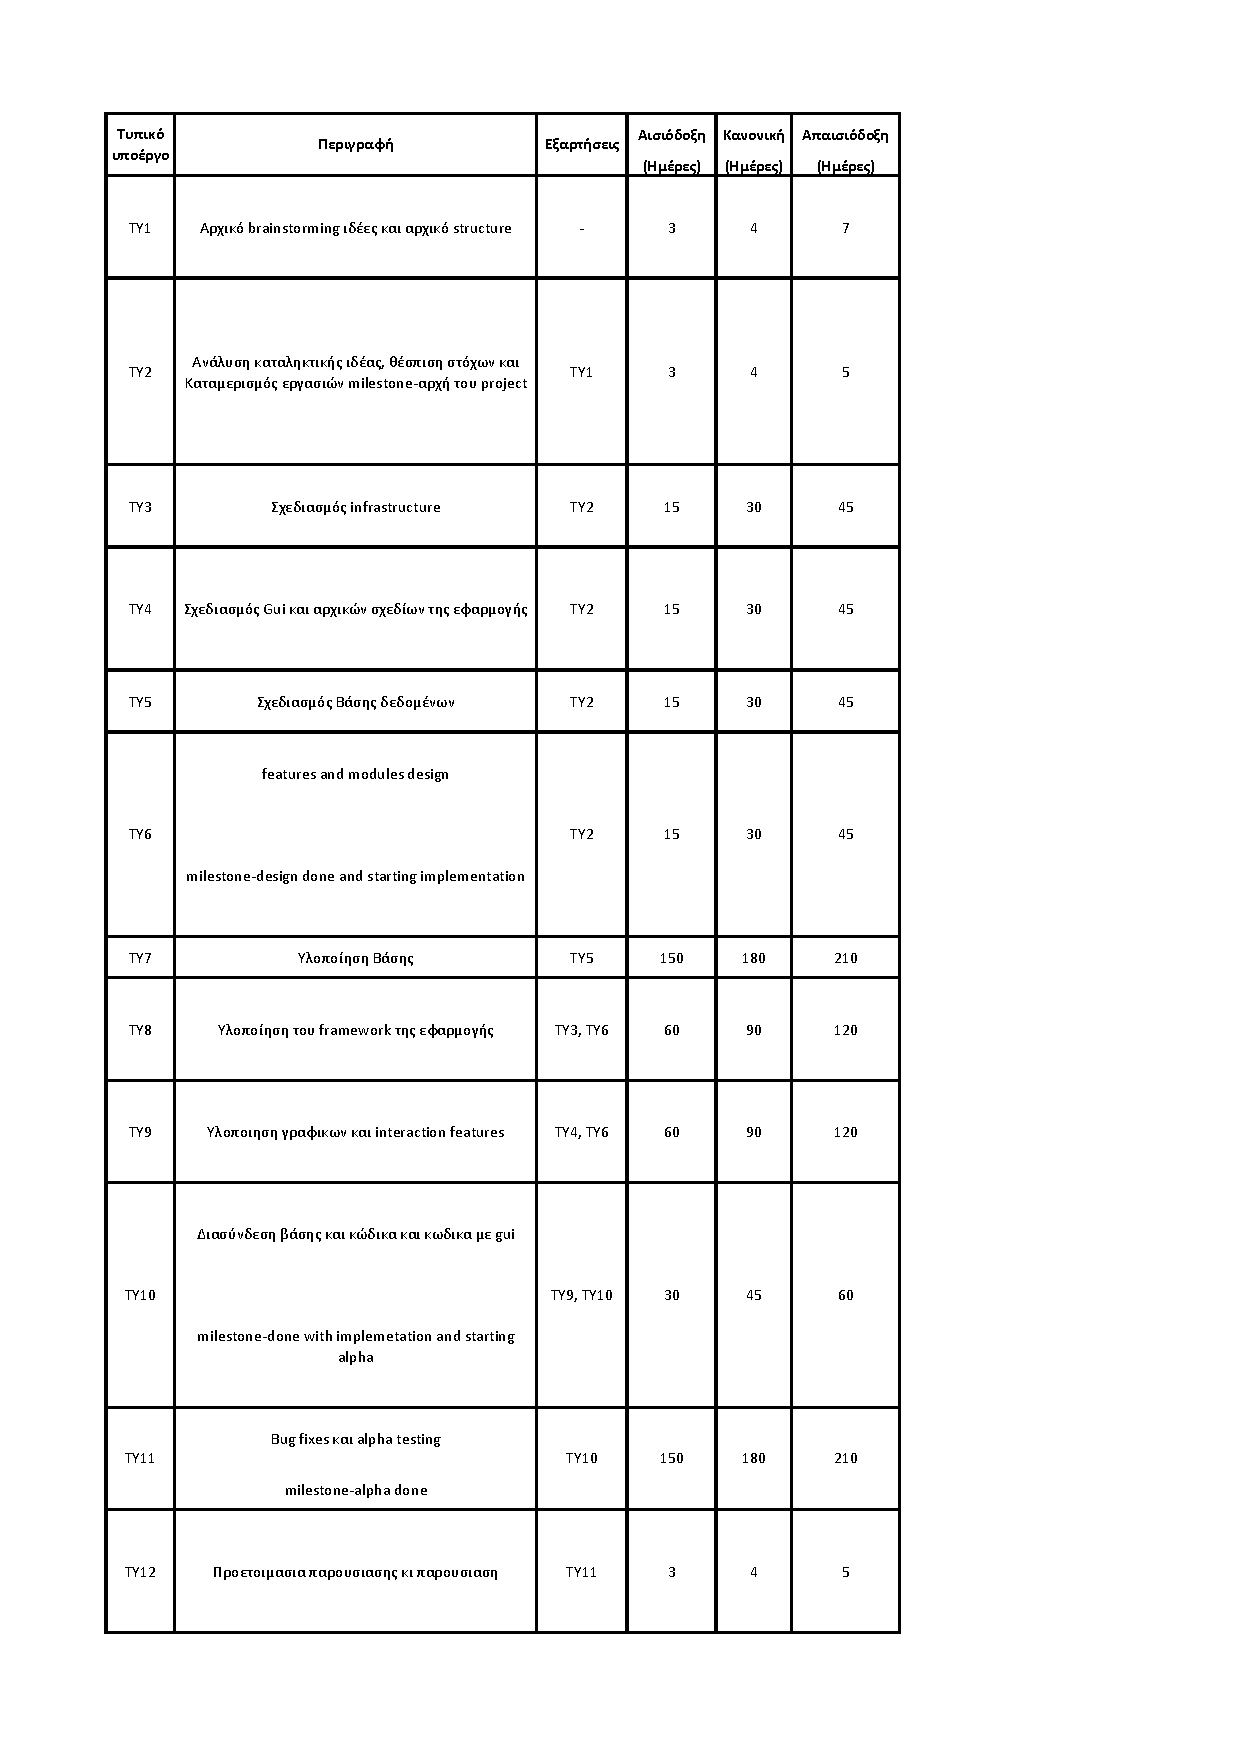
\includegraphics[width = 1.2\linewidth,trim = 0cm 2cm 0cm 1.8cm, clip]{assets/Scheduling.pdf}
% \end{figure}
% \pagebreak

\begin{table}[h]
    \hspace{-1.5cm}
    \begin{tabular}{|c|p{0.4\linewidth}|c|c|c|c|}
    \hline
        Τυπικό υποέργο & Περιγραφή & Εξαρτήσεις & Αισιόδοξη & Κανονική & Απαισιόδοξη \\
        ~ & ~ & ~ & (Ημέρες) & (Ημέρες) & (Ημέρες) \\ \hline
        ΤΥ1 & Aρχικό brainstorming ιδέες και αρχικό structure & - & 3 & 4 & 7 \\ \hline
        TΥ2 & Aνάλυση καταληκτικής ιδέας, θέσπιση στόχων και Kαταμερισμός εργασιών milestone-αρχή του project & ΤΥ1 & 3 & 4 & 5 \\ \hline
        TΥ3 & Σχεδιασμός infrastructure & ΤΥ2 & 15 & 30 & 45 \\ \hline
        TΥ4 & Σχεδιασμός Gui και αρχικών σχεδίων της εφαρμογής & ΤΥ2 & 15 & 30 & 45 \\ \hline
        TΥ5 & Σχεδιασμός Βάσης δεδομένων & ΤΥ2 & 15 & 30 & 45 \\ \hline
        TΥ6 & features and modules design & TΥ2 & 15 & 30 & 45 \\ \hline
        ~ & milestone-design done and starting implementation & ~ & ~ & ~ & ~ \\ \hline
        TΥ7 & Υλοποίηση Βάσης & TΥ5 & 150 & 180 & 210 \\ \hline
        TΥ8 & Υλοποίηση του framework της εφαρμογής & TΥ3, TY6 & 60 & 90 & 120 \\ \hline
        TΥ9 & Υλοποιηση γραφικων και interaction features & ΤΥ4, TY6 & 60 & 90 & 120 \\ \hline
        TΥ10 & Διασύνδεση βάσης και κώδικα και κωδικα με gui & ΤΥ9, TY10 & 30 & 45 & 60 \\
        ~ & milestone-done with implemetation and starting alpha & ~ & ~ & ~ & ~ \\ \hline
        TΥ11 & Bug fixes και alpha testing  & ΤΥ10 & 150 & 180 & 210 \\
        ~ & milestone-alpha done & ~ & ~ & ~ & ~ \\ \hline
        TΥ12 & Προετοιμασια παρουσιασης κι παρουσιαση & ΤΥ11 & 3 & 4 & 5 \\ \hline
    \end{tabular}
\end{table}
\pagebreak

\section{Gantt Chart}

\begin{figure}[ht]
    \hspace{-3.3cm}
    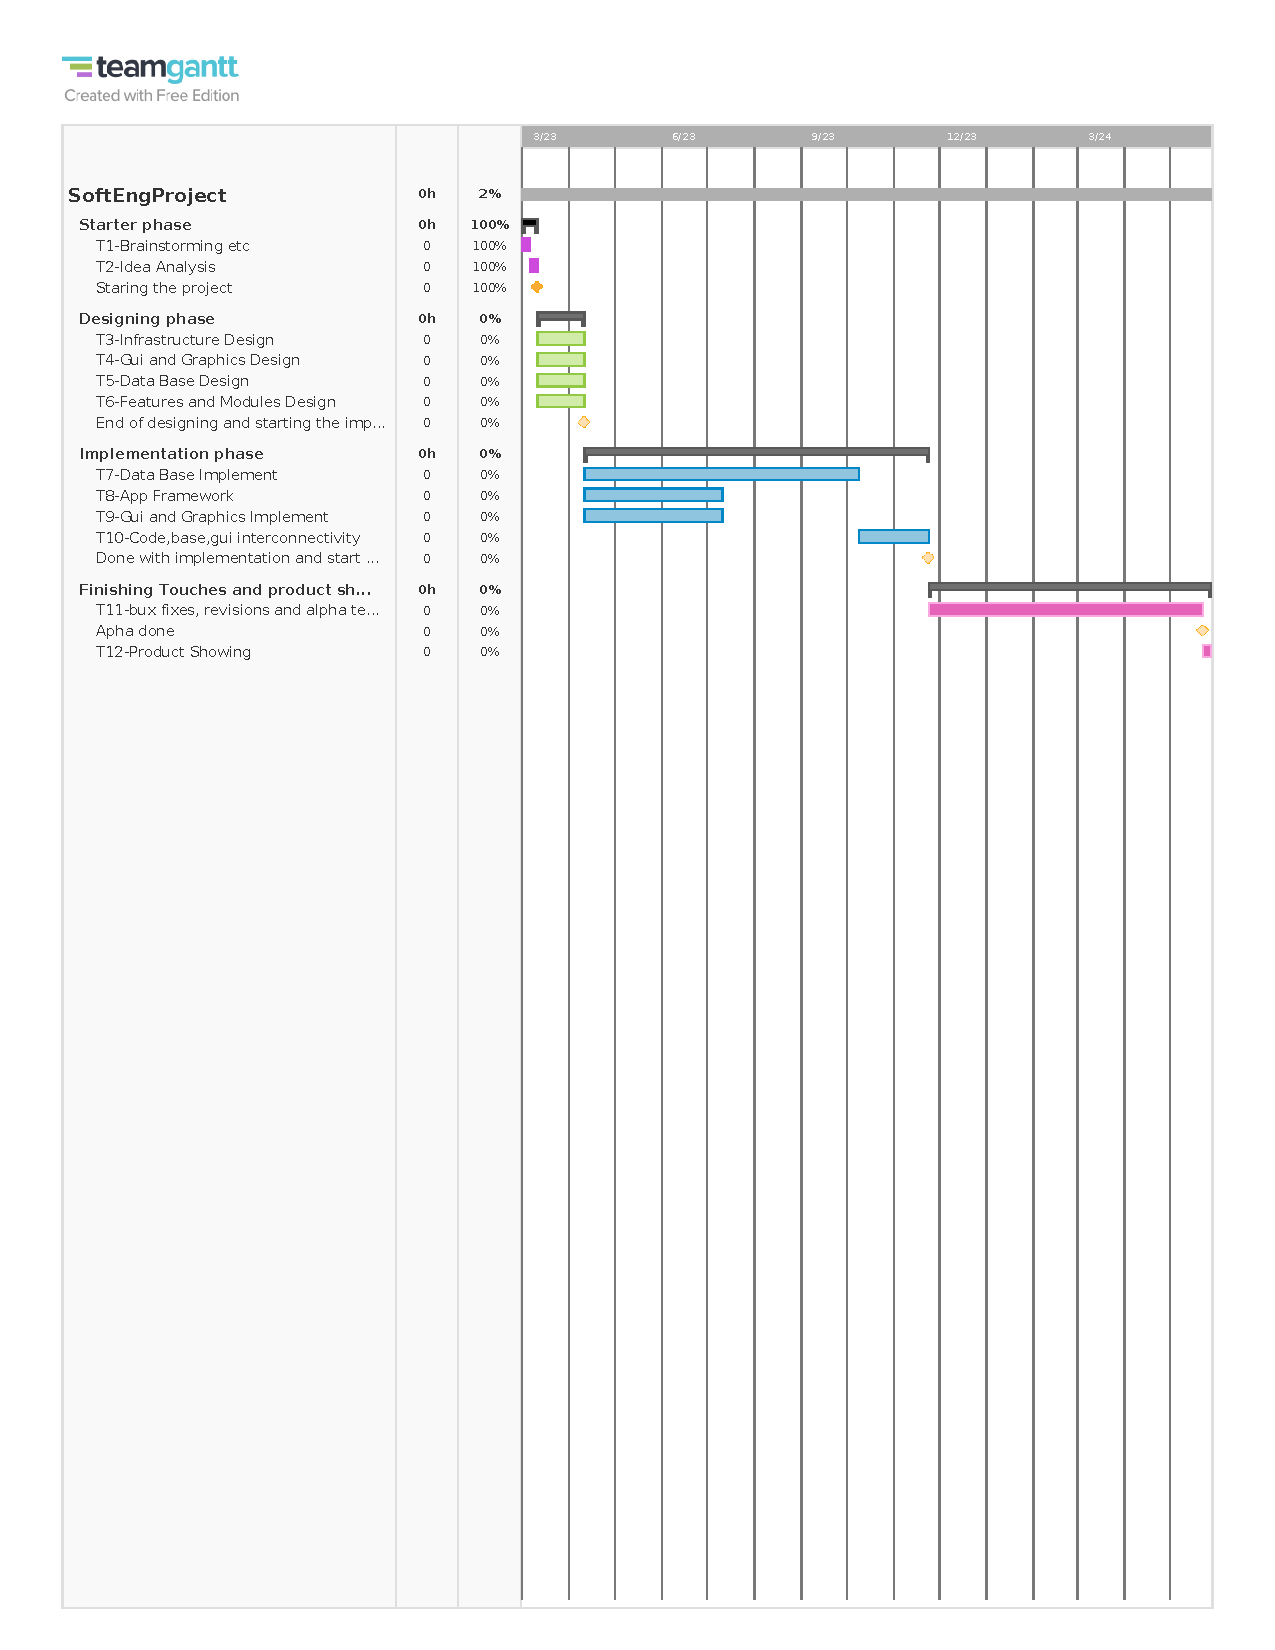
\includegraphics[trim = 0cm 12cm 0cm 2cm, clip]{assets/GanttForActualJob.pdf}
    \caption{Gantt chart}
\end{figure}
\pagebreak

\section{Pert Chart}
\begin{figure}[ht]
    \hspace{-1.7cm}
    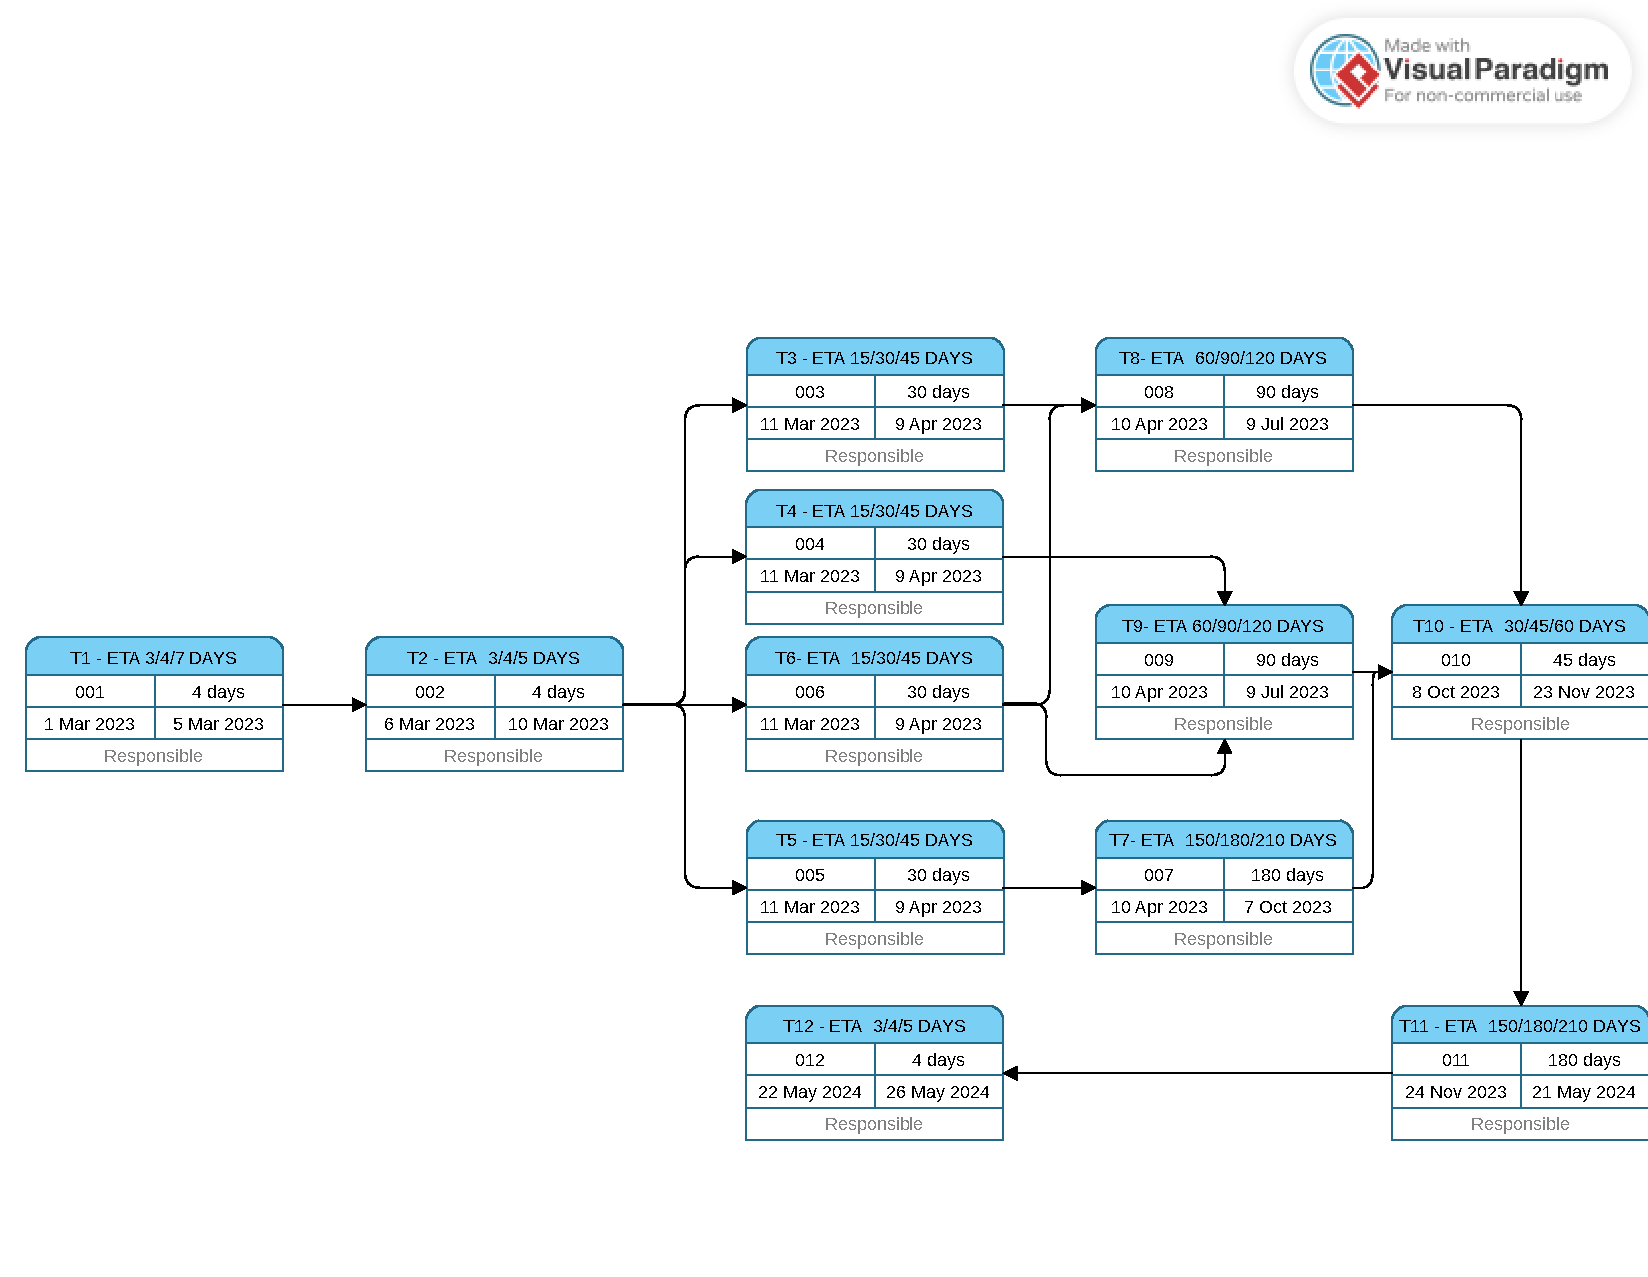
\includegraphics[width = 1.2\linewidth,trim = 0cm 0cm 0cm 3cm, clip]{assets/PertForActualJob.pdf}
    \caption{Pert chart}
\end{figure}

\section{Budget}
Με την θεώρηση, οτι αποτελούμε μέλος μιας νεοσύστατης εταιρίας, με μοναδικά μέλη εμάς,
δημιουργήσαμε ένα budget του ύψους των 84.000€, για διάστημα 15 μηνών. Έχουμε χωρίσει τον Προϋπολογισμό μας σε Άμεσά και Έμεσα Κόστη.
\pagebreak

\subsection{Άμεσα Κόστη}
Στα ΄Αμεσα κόστη έχουμε τοποθετήσει μόνο τους μισθούς των μελών της ομάδας, καθώς δεν υπολογίζεται η βοήθεια από "ἑξωτερικούς" παράγοντες.

\begin{table}[!ht]
    \centering
    \begin{tabular}{|l|l|l|l|}
    \hline
        \textbf{ΜΕΛΟΣ} & \textbf{ΜΙΣΘΟΣ} & \textbf{ΔΙΑΘΕΣΙΜΟΤΗΤΑ} & \textbf{ΣΥΝΟΛΟ} \\ \hline
        Τσούλος & 1.000€ & 100\% & 15.000€ \\ \hline
        Γιακαλλής & 1.000€ & 100\% & 15.000€ \\ \hline
        Χαλκιόπουλος & 1.000€ & 100\% & 15.000€ \\ \hline
        Παναρίτης & 1.000€ & 100\% & 15.000€ \\ \hline
        Σύνολο & 4 & ~ & 60.000€ \\ \hline
    \end{tabular}
\end{table}

\subsection{Έμμεσα Κόστη}
Στα έμμεσα κόστη, έχουν συμπεριληφθεί λειτουργικά φύσης έξοδα. 
Υποσημείωση: Η τιμή της ΔΕΗ έχει βασιστεί στις τιμές του σήμερα.


\begin{table}[!ht]
    \centering
    \begin{tabular}{|c|c|c|}
    \hline
        \textbf{ΠΑΡΟΧΕΣ} & \textbf{ΚΩΣΤΟΛΟΓΗΣΗ€} & \textbf{ΣΥΝΟΛΟ€} \\ \hline
        Γραφείο & 450€ & 6.750€ \\ \hline
        Επίπλωση & 2.000€ & 2.000€ \\ \hline
        Λειτουργικά έξοδα &    ~           &   ~      \\ 
        (ΔΕΗ, ΔΕΥΑΠ, ΟΤΕ) & (700+30+100) € & 12.450 € \\ \hline
        Τεχνολογική κάλυψη & ~             & ~ \\
        (PC, Projectors, Περιφερειακά ) & (2.000+200+500) € & 2.700€ \\ \hline
        Σύνολο & ~ & 23.900€ \\ \hline
    \end{tabular}
\end{table}

\section{Tools Used}

\begin{itemize}
    \item Συγγραφή Κειμένου: Overleaf
    \item Δημιουργία Gantt: Teamgantt
    \item Δημιουργία Pert: Visual paradigm
    \item Πίνακες: Microsoft Excel
\end{itemize}


% \bibliography{bibliography}

\end{document}
